%%%% 原overleaf模板参考北师大的LeyuDame
\documentclass[11pt]{article}
% disable indent globally
\setlength{\parindent}{0pt}
% some general improvements, defines the XeTeX logo
\usepackage{xltxtra}
\usepackage{bookmark}
% use hyperlink for email and url
\usepackage{hyperref}
\hypersetup{hidelinks}
\usepackage{url}
\urlstyle{tt}
\usepackage{multicol}
\usepackage{comment}
\usepackage{xcolor}
%%%% 统一改成了学校的蓝色，尽显专业
\definecolor{CVBlue}{RGB}{0,166,214} % 从校徽上取色

%%% \widthof[]{} 用于特殊对齐是用到
\usepackage{calc}
%%%% 利用tikz来定位照片和学校Logo
\usepackage{graphicx}
\usepackage{tikz}
\usetikzlibrary{calc}
% loading fonts
\usepackage{fontspec}
%\usepackage{xeCJK}
%\CJKsetecglue{} %% 取消中文与数字之间间隙

\setmainfont[
Path = Font/,
  Extension = .otf ,
  BoldFont = HelveticaNeueLTPro-Md.otf ,
]{HelveticaNeueLTPro-Roman.otf}
%\setCJKmainfont[
%Path = Font/,
%  Extension = .otf ,
%BoldFont=ProGB18030 DemiBold.otf,
%]{ProGB18030.otf}
%%%%% 定义更漂亮的"C++"，参考https://tex.stackexchange.com/questions/4302/prettiest-way-to-typeset-c-cplusplus 
%%%%% 貌似跟具体字体大小有关，需要调下参数，我测试感觉下面的比较好看
\usepackage{relsize}
\usepackage{xspace}
\protected\def\Cpp{{C\nolinebreak[4]\hspace{-.05em}\raisebox{.28ex}{\relsize{-1}++}}\xspace} 
% use fontawesome
\usepackage{fontawesome}
%\newfontfamily{\FA}{[FontAwesome.otf]}
\usepackage[
	a4paper,
	left=1.2cm,
	right=1.2cm,
	top=1.5cm,
	bottom=1cm,
	nohead
]{geometry}
\renewcommand{\baselinestretch}{1.2} %定义行间距1.2
\usepackage{titlesec}
\usepackage{enumitem}
\setlist{noitemsep} % removes spacing from items but leaves space around the whole list
%\setlist{nosep} % removes all vertical spacing within and around the list
\setlist[itemize]{topsep=0.25em, leftmargin=*}
\setlist[enumerate]{topsep=0.25em, leftmargin=*}
\titleformat{\section}         % Customise the \section command 
  {\large\bfseries\raggedright} % Make the \section headers large (\Large),
                               % small capitals (\scshape) and left aligned (\raggedright)
  {}{0em}                      % Can be used to give a prefix to all sections, like 'Section ...'
  {}                           % Can be used to insert code before the heading
  [{\color{CVBlue}\titlerule}]                 % Inserts a horizontal line after the heading
\titlespacing*{\section}{0cm}{*1.6}{*1.2}
\usepackage{siunitx}
\usepackage{amssymb}
%\xeCJKsetup{CJKspace=true}
%\xeCJKDeclareCharClass{CJK}{`0 -> `9}    % 设置 0-9 以 CJK 字体输出
%\normalspacedchars{0,1,2,3,4,5,6,7,8,9} % 0-9 的字符类被还原


\begin{document}

\pagenumbering{gobble} % suppress displaying page number
%%%% 利用tikz来定位照片，部分招聘单位可能需要"以貌取人"
\begin{tikzpicture}[remember picture, overlay]
	\node[anchor = north east] at ($(current page.north east)+(-1cm,-1.2cm)$) {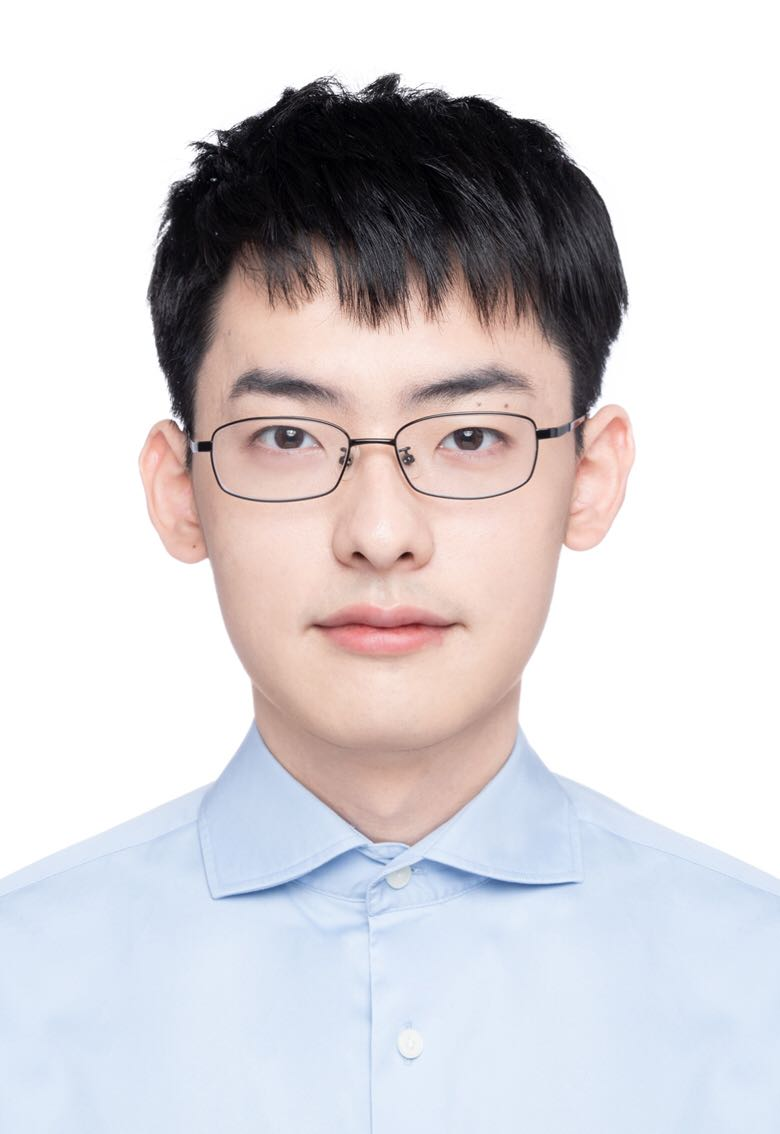
\includegraphics[height=3.8cm]{img/photo.jpg}};
\end{tikzpicture}%

%%%% 利用tikz来定位学校Logo，这里只在第一页显示，如果需要每页都有，可以考虑在页眉、页脚或者background中加入，不过简历也就一两页，无所谓了

\begin{tikzpicture}[remember picture, overlay]
	\node[anchor = north west] at ($(current page.north west)+(0.2cm,-0.2cm)$) {
\includegraphics[height=3.5cm]{img/international-logo_rgb@16x.png}};
\end{tikzpicture}%

%%%% 利用tikz来定位页脚栏，电子版简历使用，黑白纸质打印效果可能并不好。这里只在第一页显示，如果需要每页都有，页脚或者background中加入。

%\begin{tikzpicture}[remember picture, overlay] 
%    \node[anchor = south,fill=CVBlue,draw=none,minimum width=\paperwidth,minimum height=1.5em,align=center,font=\footnotesize,text=white] at ($(current page.south)$) 
%    {\faGithubAlt \ \href{https://github.com/leyudame}{https://github.com/leyudame}\qquad
%        \faRssSquare \ \href{https://leyudame.github.io}{https://leyudame.github.io} };
%\end{tikzpicture}

%tikzpicture环境很敏感，注释周围的空格、空行都会引起水平距离或垂直距离的变化，
%
\centerline{\LARGE\bfseries{Xiaoyun Qian}}

%\centerline{\normalsize{Target Position: Analog IC Design \quad Major: Microelectronics}}
\centerline{\normalsize{Major: Microelectronics}}
\centerline{\normalsize{
    \faPhone \ +86 13816092395 \quad
    \faPhone \ +31 682320671 \quad
    \faEnvelopeO \ \href{mailto:qianxiaoyun2000@outlook.com}{qianxiaoyun2000@outlook.com}}}


\section{\makebox[\widthof{\faGraduationCap}][c]{\color{CVBlue}\faGraduationCap}\  Education}

\textbf{Delft University of Technology} (September 2023 -- Present)

\qquad M.Sc. Student \quad Microelectronics,  
\quad Thesis: \emph{Design of an Energy-Efficient Multichannel Neural Stimulation System for Wireless Visual Cortex Stimulation}, Expected July 2026

\textbf{HZ University of Applied Sciences, the Netherlands} (February 2022 -- July 2023)

\qquad Bachelor of Engineering (HBO)  
\quad Thesis: \emph{Design and Manufacturing of a Battery Pack Clamping System with Integrated Vision Positioning for Laser Welding}

\textbf{Shanghai Maritime University} (September 2019 -- July 2023)

\qquad Bachelor of Engineering \quad Mechatronics Engineering



\begin{comment}

\end{comment}

\section{\makebox[\widthof{\faGraduationCap}][c]{\color{CVBlue}\faBriefcase}\ Work Experience}
    \begin{itemize}
    \item \textbf{Shanghai United Imaging Healthcare Co., Ltd.} (July--August 2025), Shanghai, China, Intern
    \begin{itemize}
    \item Participated in PET medical imaging sensor development in the MI-DET-DEA department, contributing to the ``Kunpeng'' and ``Qilin'' projects
    \item Conducted electromagnetic shielding performance testing and failure analysis of sensors, identified EMI interference sources, and proposed improvement solutions to enhance signal integrity
    \item Executed vibration testing for ``Kunpeng'' and environmental stress testing for ``Qilin'' (Kunshan laboratory), participated in failure analysis and assisted design optimization to verify medical-grade reliability
    \end{itemize}

	\item \textbf{EmergoStar B.V.} (January--August 2023), Terneuzen, the Netherlands, Electrical Engineer
    \begin{itemize}
    \item Designed a battery pack clamping system capable of withstanding 3000\,N clamping force, optimized the structure through mechanical simulation to improve battery lifespan
    \item Fabricated test tools using 3D printing and integrated a vision positioning system into a laser welding platform, enabling precise positioning and modular improvements
    \item Developed a pressure sensor testing platform using Arduino, enabling real-time monitoring of clamping force distribution, validating system performance, and reducing assembly changeover time by over 30\%
\end{itemize}
	\item \textbf{Lumileds (Shanghai) Management Co., Ltd.} (July--August 2021), Shanghai, China, Intern
    \begin{itemize}
    \item Performed high-precision mounting of semiconductor light source chips using microscopes and thermocompression soldering tools, gaining experience in precision soldering processes
    \item Conducted driving tests using constant-current power supplies and fabricated engineering samples for customer demonstrations of LED performance
    \item Maintained and updated the company’s internal product data server, providing update logs and user documentation
    \end{itemize}
\end{itemize}


\section{\makebox[\widthof{\faGraduationCap}][c]{\color{CVBlue}\faUniversity}\ Projects}
\begin{itemize}
\item \textbf{Design of an Energy-Efficient Multichannel Neural Stimulation System for Wireless Visual Cortex Stimulation} (September 2025 -- July 2026, Ongoing)
    \begin{itemize}
    \item \textbf{System Architecture}: Designed an 8-channel neural stimulation ASIC supporting 1:8 time-division multiplexing (TDM) to drive 64 electrodes, with SPI-based channel configuration for wirelessly powered cortical visual prosthesis applications
    \item \textbf{Low-Power Hierarchical Biasing Architecture}: Implemented a global bias block distributing gate voltages to per-channel current mirrors, achieving approximately 20\,µW static power consumption per channel
    \item \textbf{PI Closed-Loop Controller}: Replaced the original open-loop amplifier architecture to eliminate steady-state error and improve system stability during load switching
    \item \textbf{Active-Feedback IDAC}: Isolated high voltage via op-amp output clamping; employed 2\,V devices in the second-stage cascode to improve speed, reducing headroom from 250\,mV to 60\,mV (76\% reduction)
    \item \textbf{Idle Controller}: Detected excess voltage headroom and automatically disabled the PI controller and comparator to optimize efficiency during high-to-low load transitions
    \item \textbf{CMLS-Based Level Shifter}: Resolved insufficient rising-edge speed in the original cross-coupled architecture, optimizing rectifier switch control signals from glitch-prone waveforms to clean square waves
    \item \textbf{Complementary NMOS Rectifier Switch}: Automatically switched to NMOS conduction under low-voltage conditions, achieving a 150\% efficiency improvement at 5\,µA / 20\,kΩ load
    \item \textbf{VCDL Optimization}: Optimized delay tuning range from 33\,ns--800\,ps to 10\,ns--170\,ps (70\% reduction in minimum delay), enabling fast TDM switching
    \item \textbf{Performance}: Output current 0--155\,µA (5\,µA step), load resistance 20--70\,kΩ, support for 1--20\,nF capacitive loads; overall efficiency superior to the original system and operational down to 5\,µA; robustness verified via Monte Carlo and four process-corner simulations
    \item \textbf{Current Status}: Circuit design and core layout completed; tape-out scheduled for April 20, 2026
    \end{itemize}

    \item \textbf{BiCMOS Process Fabrication and Device Characterization Laboratory} (2025)
    \begin{itemize}
        \item Completed a full BiCMOS fabrication flow including thermal oxidation, ion implantation, lithography, wet and dry etching, and metallization
        \item Performed process and device simulations using Synopsys Sentaurus to predict doping profiles and electrical characteristics
        \item Characterized NMOS/PMOS devices using a Keysight B1500A semiconductor parameter analyzer, extracting threshold voltage, mobility, and subthreshold swing
        \item Conducted sheet resistance measurements, ELM measurements, and lateral diffusion analysis to validate simulation model accuracy
    \end{itemize}

    \item \textbf{High-Precision Residue Amplifier Design} (2024--2025)
    \begin{itemize}
        \item Designed a two-stage fully differential amplifier achieving 66\,dB SNR, 80.33\,dB gain, and 24.88\,ns settling time
        \item Developed Python scripts to automate LTspice simulations, enabling parameter extraction, design space exploration, and iterative optimization
        \item Applied Miller compensation to optimize frequency response; reduced power consumption to 0.828\,mW through noise--bandwidth trade-offs, achieving a FoM of $-173.8$\,dB
        \item Designed complete common-mode feedback and bias networks; completed transient analysis, noise analysis, and performance verification
    \end{itemize}

    \item \textbf{Kaggle Titanic -- Machine Learning from Disaster} (2023)
    \begin{itemize}
        \item Built deep learning models using PyTorch to predict Titanic passenger survival, including feature engineering and data preprocessing
        \item Compared multiple machine learning algorithms and optimized hyperparameters to improve model performance
        \item Achieved final ranking of 559 / 14{,}393 (Top 4\%) with an accuracy of 0.799
    \end{itemize}
\end{itemize}


\section{\makebox[\widthof{\faGraduationCap}][c]{\color{CVBlue}\faWrench}\ Skills}

\begin{itemize}
	\item Languages: English (CET-4, CET-6), Japanese (JLPT N4), Dutch (A1)
	\item Programming: Python, PyTorch (Kaggle Titanic ranking 559/14393), \Cpp, \LaTeX, \ldots
	\item Professional Tools: LTspice, Cadence, MATLAB, HSPICE, Jupyter Notebook, SolidWorks, Arduino

\end{itemize}

%\section{\makebox[\widthof{\faGraduationCap}][c]{\color{CVBlue}\faTags}\ Others}
% increase linespacing [parsep=0.5ex]
%Hobbies and Interests: Pursuing PhD


%%%% 如果多页简历,可以手动在适当位置插入 \newpage 或者 \clearpage 开始新一页

\end{document}